\documentclass{InsightArticle}

\usepackage[dvips]{graphicx}
\usepackage{float}
\usepackage{subfigure}
%\usepackage{l2tabu}
%\usepackage{lstlisting}

\usepackage[dvips,
bookmarks,
bookmarksopen,
backref,
colorlinks,linkcolor={blue},citecolor={blue},urlcolor={blue},
]{hyperref}

\title{Moore Neighbor Tracing}

% 
% NOTE: This is the last number of the "handle" URL that 
% The Insight Journal assigns to your paper as part of the
% submission process. Please replace the number "1338" with
% the actual handle number that you get assigned.
%
\newcommand{\IJhandlerIDnumber}{3308}

% Increment the release number whenever significant changes are made.
% The author and/or editor can define 'significant' however they like.
\release{0.00}

% At minimum, give your name and an email address.  You can include a
% snail-mail address if you like.

\author{David Doria}
\authoraddress{Rensselaer Polytechnic Institute}


\begin{document}

\IJhandlefooter{\IJhandlerIDnumber}


\ifpdf
\else
   %
   % Commands for including Graphics when using latex
   % 
   \DeclareGraphicsExtensions{.eps,.jpg,.gif,.tiff,.bmp,.png}
   \DeclareGraphicsRule{.jpg}{eps}{.jpg.bb}{`convert #1 eps:-}
   \DeclareGraphicsRule{.gif}{eps}{.gif.bb}{`convert #1 eps:-}
   \DeclareGraphicsRule{.tiff}{eps}{.tiff.bb}{`convert #1 eps:-}
   \DeclareGraphicsRule{.bmp}{eps}{.bmp.bb}{`convert #1 eps:-}
   \DeclareGraphicsRule{.png}{eps}{.png.bb}{`convert #1 eps:-}
\fi


\maketitle


\ifhtml
\chapter*{Front Matter\label{front}}
\fi

\begin{abstract}
\noindent

This document presents an implementation of Moore Neighbor Tracing - an algorithm to find an ordered outline of a blob or contour in an image.

An excellent tutorial on Moore Neighbor Tracing is provided here:
\verb|http://www.imageprocessingplace.com/downloads_V3/root_downloads/|
\verb|tutorials/contour_tracing_Abeer_George_Ghuneim/moore.html|


The code is available here:
\verb|https://github.com/daviddoria/MooreTracing|

\end{abstract}

\IJhandlenote{\IJhandlerIDnumber}

\tableofcontents
%%%%%%%%%%%%%%%%%%%%
\section{Introduction}
This document presents an implementation of Moore Neighbor Tracing - an algorithm to find an ordered outline of a blob in an image. The algorithm also works for images already containing contours (non-filled blobs) in that it assigns an ordering to the contour pixels.

An excellent tutorial on Moore Neighbor Tracing is provided here:

\verb|http://www.imageprocessingplace.com/downloads_V3/root_downloads/|
\verb|tutorials/contour_tracing_Abeer_George_Ghuneim/moore.html|

This particular implementation is designed to be used with a ``label image'', typically the output of a pipeline consisting of one of many filters that produces an itkLabelMap (e.g. itkBinaryImageToLabelMapFilter) followed by a itkLabelMapToLabelImageFilter. Therefore, since we are looking to order the pixels in an already-known-to-be closed blob or contour, the termination criterion that has been implemented is returning to the starting pixel. Moore Neighbor Tracing can also be used with other stopping criteria to order pixels of open contours.

The code is available here:
https://github.com/daviddoria/MooreTracing

%%%%%%%%%%%%%%%%%%%%
\section{Algorithm}
The algorithm proceeds as follows:

Initialization:
\begin{enumerate}
\item Locate a boundary pixel. This can be found simply using a raster scan of the image and looking for the first non-background pixel.
\end{enumerate}

Iterate:
\begin{enumerate}
  \item Start on a boundary pixel. This can be found simply using a raster scan of the image and looking for the first non-background pixel.
 \item Record the pixel from which you ``entered'' the contour pixel.
 \item Traverse the 8-connected neighbors (consistently either clockwise or counter-clockwise), looking for another non-background pixel. The direction of the contour will be the same as the choice of the neighborhood traversal direction (either clockwise or counterclockwise). We have arbitrarily chosen counter-clockwise traversal in this implementation.
\end{enumerate}

Termination:
\begin{enumerate}
 \item Terminate when the initial pixel is reached.
\end{enumerate}

%%%%%%%%%%%%%%%
\section{Implementation}
This implementation only traces the first contour found in an image. If the image contains more than one contour, the user could remove the pixels found in the first contour and then call MooreTrace until there are no more contours.

%%%%%%%%%%%%%%%
\section{Example}
Figure \ref{fig:Example} shows the computed ordering of the pixels on a square. The tracing started in the top left corner and proceeded counter-clockwise around the square.

\begin{figure}[H]
\centering
\subfigure[Input image.]
  {
  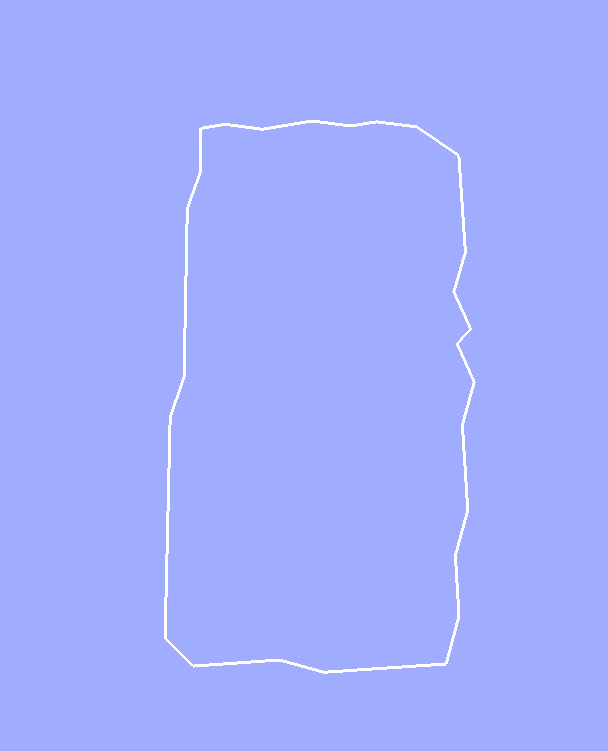
\includegraphics[width=0.3\linewidth]{images/input}
  \label{fig:1Iteration:Original}
  }
\subfigure[Output image showing the ordering of pixels (black to white (i.e. Hot colormap)).]
  {
  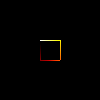
\includegraphics[width=0.3\linewidth]{images/output}
  \label{fig:1Iteration:1Erosion}
  }
\caption{Example of Moore Neighbor Tracing.}
\label{fig:Example}
\end{figure}

%%%%%%%%%%%%%%%
\section{Code Snippet}

\begin{verbatim}
  // Create an image
  ImageType::Pointer image = .... obtain an image from somewhere ....
  
  // Trace the contour
  std::vector< itk::Index<2> > path = MooreTrace(image);
  
  // Output the ordered contour pixels
  for(unsigned int i = 0; i < path.size(); ++i)
    {
    std::cout << path[i] << std::endl;
    }
\end{verbatim}


\end{document}